
The analysis relies on the selection of electrons, muons, jets and $b$-tagged jets. This chapter reviews the reconstruction, definition, efficiencies and calibration of these objects in ATLAS.
\section{Track reconstruction}
Measurements from the three subdetectors of the ID are combined to make \emph{tracks}, a description of the trajectory and momentum of each charged particle. The algorithm begins by finding track seeds in the inner silicon layers obtained by a window search algorithm. These seeds are then reconstructed into tracks with the ATLAS tracking algorithm\cite{ATLAS-CONF-2012-042}.

The algorithm works first from the inside of the detector outward. Pattern recognition is used to make the pixel detector seeds into three-point track candidates. Then, a Kalman filter is used to add SCT hits radially outward. After ambiguities such as missing or shared hits are resolved, the tracks are extended into the TRT. Tracks are required to have $\pt > 400 \mev$ to be reconstructed. This cut was introduced to reduce the computation time for the pattern recognition algorithm. After this inside-out algorithm as been completed, an outside-in algorithm is run on the unused hits, to reconstruct secondary tracks left by particles not originating directly from the IP, for example kaon and lambda decay products.

Since charged particle tracks are bent by the magnetic field, the trajectory takes a helical form and can be expressed by 5 parameters: 
\begin{description}
\item[$d_0$:] the transverse impact parameter, equal to the distance of closest approach in the plane transverse to the beam of the track to the primary vertex
\item[$z_0$:] the longitudinal impact parameter, equal to the $z$ coordinate of the point of closest approach to the primary vertex
\item[$\phi_0$:] the azimuthal angle of the trajectory at the point of closest approach to the primary vertex
\item[$\cos\theta$:] the cosine of the angle the track forms with respect to the beam
\item[$q/p_T$:] the charge divided by the momentum in the transverse plane.
\end{description}



\section{Primary vertex reconstruction}
A primary vertex reconstruction algorithm determines if many tracks originate from the same $pp$ collision\cite{ATLAS-CONF-2010-069,ATLAS-CONF-2012-042}. The vertices are reconstructed with an iterative fitting procedure. Initially, a vertex seed is created from a fit to the global maximum of the $z$ coordinates of the tracks. Then, tracks are matched to the seed using a \chisq\ algorithm. Incompatible tracks are used to seed a new vertex until all tracks are associated with a vertex.

Since several $pp$ collisions are likely to occur for each bunch crossing, some of the tracks will be associated with secondary vertices from pileup rather than the primary vertex (PV) from the hard collision. The PV is conventionally defined as the vertex with the highest track $\pt^2$. In 2012, the average number of interactions per crossing was 20.7, as shown in Figure~\ref{fig:atlas-pileup}, so primary vertex reconstruction is essential for determining which particles came from pileup. If a track isn't associated with the PV, it is typically considered pileup. Figure~\ref{fig:disppileup} shows an event with 22 vertices, demonstrating the important of tracking and vertexing in events with high pileup.


\begin{figure}[tp]
  \centering
  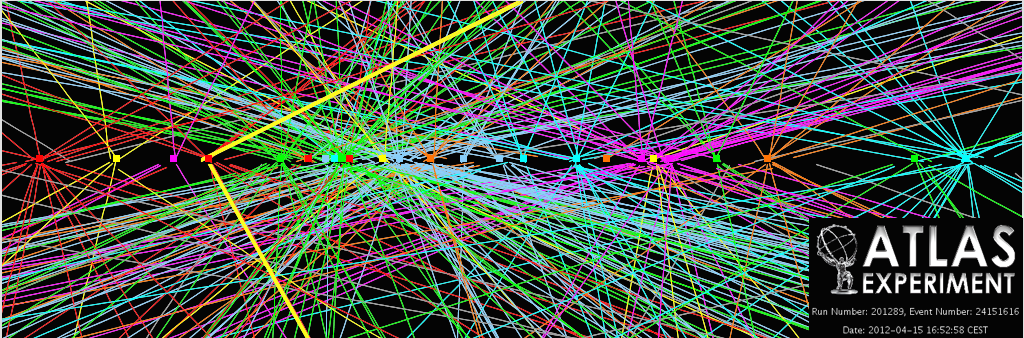
\includegraphics[width=0.95\textwidth]{fig/atlas/pileupEvent}
  \caption{Display of a 2012 event with 25 reconstructed vertices~\cite{eventdisp}.}
  \label{fig:disppileup}
\end{figure}

\section{Muons}
Muons are reconstructed by combining tracks found in the muon spectrometer and inner detector. Track segments are found in each layer of the detector then combined, taking into account energy loss while crossing the calorimeters. Tracks in the ID are required to pass minimum hit requirements in the Pixel, SCT, and TRT. Muons can be reconstructed using only the MS, but in this analysis uses \emph{combined} muons (reconstructed in both the MS and ID) to ensure high purity.

The muon reconstruction efficiency can be measured using the \emph{tag-and-probe} method. The ID reconstruction efficiency is determined from events reconstructed with one combined muon, the \emph{tag}, and a second muon only required to have an MS track, the \emph{probe}. The ID reconstruction efficiency is given by the fraction of events where the MS track probe also has a track in the ID. The same method can be used to determine the efficiency of the MS reconstruction. This time, the ID segments are used as the probe and the MS+matching efficiency is given by the fraction of ID segments with a matching MS segment. The overall muon reconstruction efficiency is given by the product of these two efficiencies. To obtain the scale factors (SF), the muon reconstruction efficiency in data and MC is compared: $SF = \epsilon_{data}/\epsilon_{MC}$. These scale factors are applied to the simulation to ensure that muons are reconstructed with the same efficiency in MC as in data. For muons, the SFs are calculated in bins of \pt\ and $\eta$ using $Z\rightarrow \mu\mu$ and $J/\Psi\rightarrow \mu\mu$ events~\cite{muonpaper}. 

The muon momentum scale and resolution of the MC must also be corrected to match data. Differences can come from mis-modeling of the detector geometry, magnetic field, or energy loss in the calorimeter. Scale factors are determined by comparing the shape of the energy distribution in $Z\rightarrow \mu\mu$ and $J/\Psi\rightarrow \mu\mu$ events. For 2012, the corrections were less than 0.1\%~\cite{muonpaper}.

Finally, the efficiency of the muon trigger is also estimated via the tag-and-probe method. In this analysis, the logical OR of two triggers is used to identify muons: a 24 GeV trigger with a loose track-based isolation requirement (the sum of the \pt of tracks within a cone of $\Delta R$=0.2 must be less than 12\% the \pt of the muon) and a 36 GeV trigger without an isolation requirement. For $\pt<100 \gev$, $Z\rightarrow\mu\mu$ events are used to estimate the trigger efficiency, while $W+$jets is used for \pt\ above this threshold. The muon trigger efficiency in the barrel region is derived from $Z\rightarrow\mu\mu$ events is shown in Figure~\ref{fig:muontrigger}.

\begin{figure}[hp]
\centering
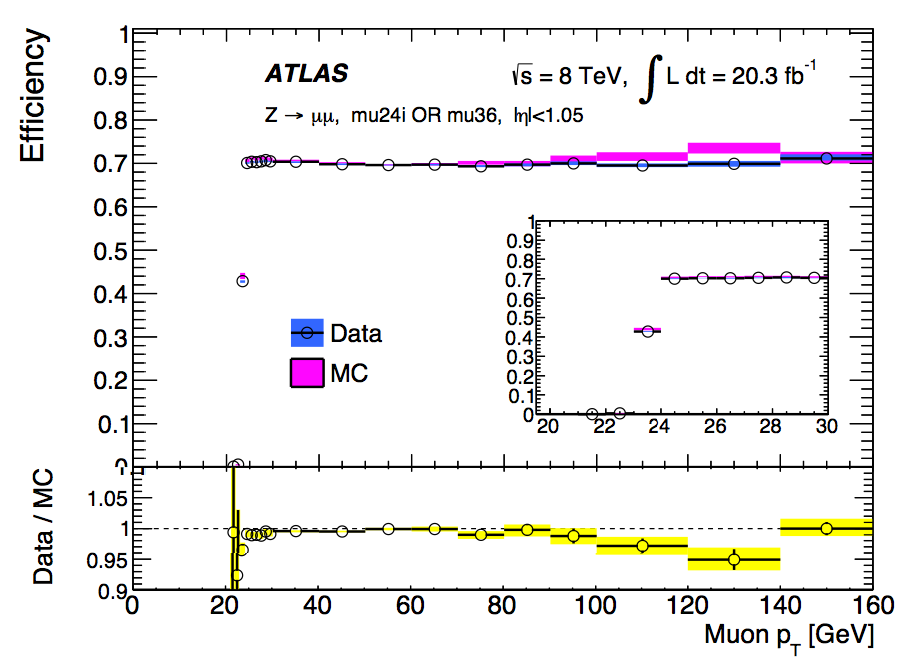
\includegraphics[width=0.6\textwidth]{fig/obj/muontrigger.png}
\caption{Reconstruction and identification efficiency for the muons as a function of \pt~\cite{Aad:2014fxa}.}
\label{fig:muontrigger}
\end{figure}

\section{Electrons}
The reconstruction of electrons uses information from both the EM calorimeters and tracks in the ID. First, clusters of energy are found using the sliding-window algorithm described in Chapter~\ref{ss:cluster}. Then, tracks reconstructed in the ID are extended into the calorimeter. Tracks and clusters are considered a match if the center of the cluster and the track are within $\Delta\eta<$0.05 and $\Delta\phi<$0.1. Clusters that don't match to a track are considered as candidate photons~\cite{Aad:2014fxa}.

Quality requirements divide electron candidates into three categories: loose, medium and tight. In this analysis, electrons are required to match the tight requirements, such as ID hit requirements, shower shape, track quality and tighter criteria for matching tracks and clusters. The total reconstruction and identification efficiency for these tight electrons is shown in Figure~\ref{fig:electronID}. As with muon reconstruction, tag-and-probe methods determine the electron reconstruction scale factors using $Z\rightarrow ee$ events.

The electron energy scale of the MC must be corrected to match data. First, the MC simulation of electron response is used as a initial calibration of the electron energy. Then, the absolute energy scale and resolution are determined by comparing $Z\rightarrow ee$ events in data and MC. This calibration is then checked against $J/\Psi\rightarrow ee$ events.

In this analysis, the logical OR of two triggers is used to identify electrons: a 24 GeV trigger with a loose track-based isolation requirement and a 60 GeV trigger without an isolation requirement. The isolation requirement specifies that the sum of the \pt of tracks within a cone of $\Delta R$=0.2 must be less than 10\% the \pt of the electron. The trigger efficiency is evaluated with a tag-and-probe of $Z\rightarrow ee$ events, using the tight electron matched to a trigger with a lower threshold as a tag and an electron with opposite charge as a probe. This efficiency is shown in Figure~\ref{fig:eltrigger}.

 The electron trigger efficiency is measured using tag-and-probe in $Z\rightarrow ee$ events, where the tag is a tight electron matched to a trigger with a lower threshold and the probe is an oppositely charged electron such that the $ee$ system has invariant mass within the $Z$ mass window of 80-100 GeV. The measured efficiency is shown in Figure~\ref{fig:eltrigger}. 

\begin{figure}[hp]
\centering
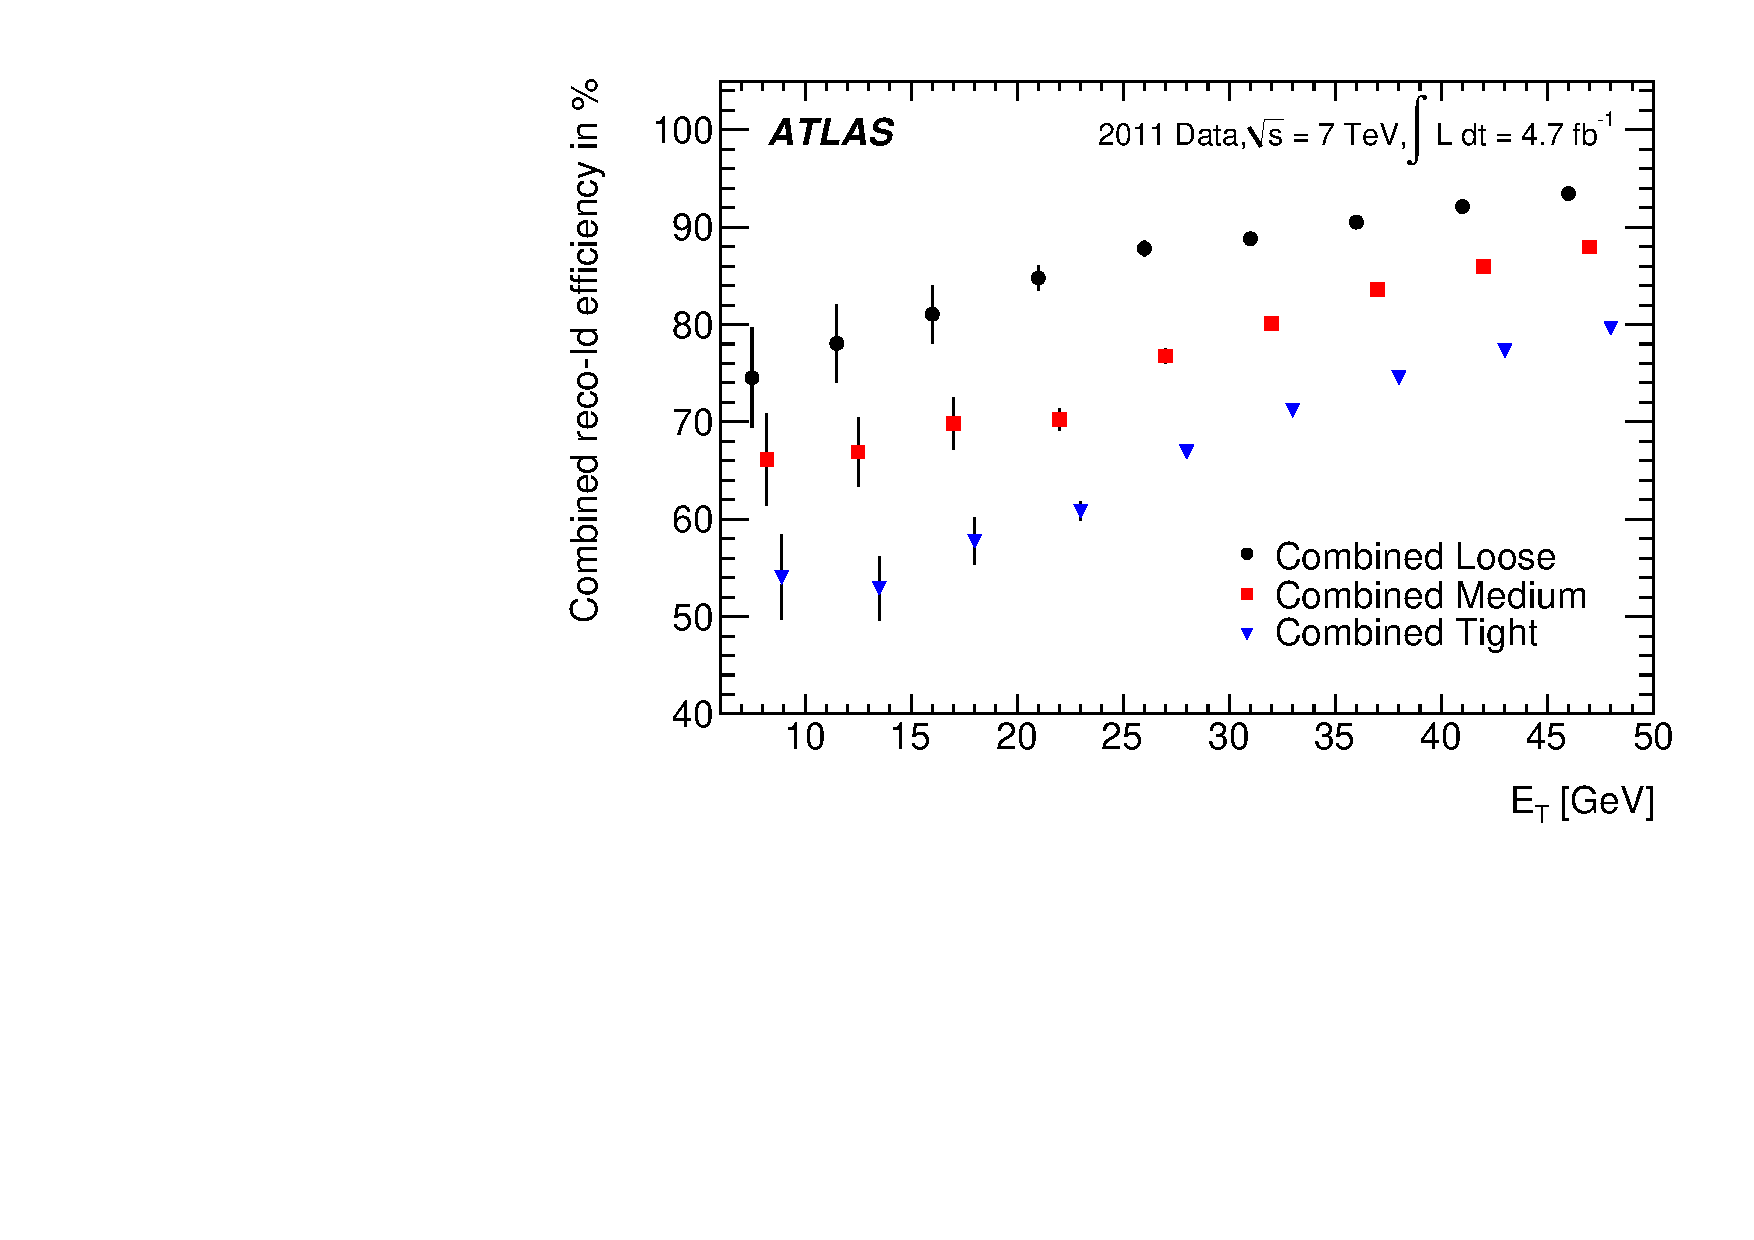
\includegraphics[width=0.6\textwidth]{fig/obj/electronID.pdf}
\caption{Reconstruction and identification efficiency for the electrons as a function of $E_{T}$~\cite{Aad:2014fxa}.}
\label{fig:electronID}
\end{figure}
\begin{figure}[hp]
\centering
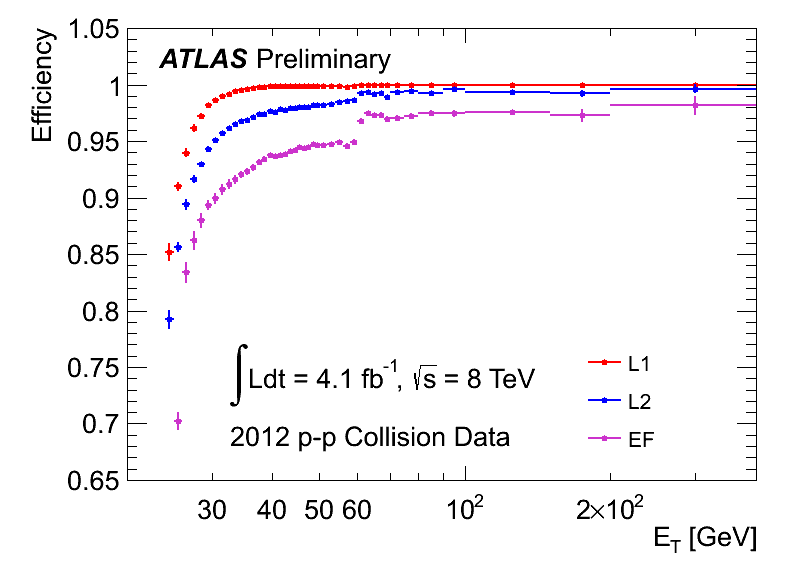
\includegraphics[width=0.6\textwidth]{fig/obj/eltrigger.png}
\caption{Combined efficiency of the 24 GeV and 60 GeV electron triggers. ~\cite{eltrig}.}
\label{fig:eltrigger}
\end{figure}

\section{Jets}
Jet reconstruction begins with the formation of \emph{topo-clusters} from energy deposits in the EM and hadronic calorimeter cells as described in Chapter~\ref{ss:cluster}. Once the clusters have been built, they are used as input to the the anti-$k_t$ algorithm~\cite{antikt1,antikt2,antikt3} with radius parameter $R=0.4$. In addition to jets from calorimeter clusters, \emph{track-jets} are also constructed from charged particle tracks for calibration purposes. The final 4-momentum of the jet is defined as the sum of the 4-momenta of its constituents. 

At this stage, the jet reconstruction efficiency and its uncertainty can be measured in data using the fraction track-jets matched to calorimeter jets. The efficiency can also be calculated using a tag-and-probe method in dijet events. The reconstruction inefficiency is found to be very small: about 0.0002\% for jets with $\pt< 20 \gev$ and negligible for jets with higher \pt.

The jets are first corrected for the effects of pileup using the jet area method~\cite{JES}. This method corrects the \pt\ of the jet by subtracting $\rho\times A$. The quantity $\rho$ is defined as the  the energy density in the event calculated from all calibrated topo-clusters within $|\eta|\leq$ 2, and the quantity $A$ is defined as the catchment area of the jet. This correction depends both on the characteristics of the jet and the pileup in the event. Then a residual correction dependent on the instantaneous luminosity and number of reconstructed primary vertices in the event is made. This correction is primarily relevant in the forward region and is derived from simulation.

The jets are then calibrated using a function that depends on both energy and $\eta$~\cite{JES}. The jet direction is corrected so that the jet originates from the primary vertex. Next, the energy scale of the jet (JES) correction is applied, which has both an MC-based and \emph{in situ} component. The energy- and $\eta$-dependent MC-based JES scheme is derived from the ratio of the energy of a detector level jet to the matching truth level jet (jets formed using the same anti-$k_t$ algorithm from simulated hadrons). The \emph{in situ} correction uses data events where a jet recoils against a $Z$ or a photon, which can be more precisely measured by the detector. However, this method can only be used for jets with $\pt<800 \gev$. Jets with $\pt>800 \gev$ are calibrated with events where a high \pt\ jet recoils against a several lower \pt\ jets already calibrated by the $Z$ or photon events. The final JES and uncertainty comes from a combination of such measurements. Figure~\ref{fig:jesex} shows the JES uncertainty for jets in the central $\eta$ region ($|\eta|<2.5$). The jet energy resolution (JER) is studied separately via a similar process with dijet events, and the resolution in data and simulation is found to be comparable.

\begin{figure}[hp]
\centering
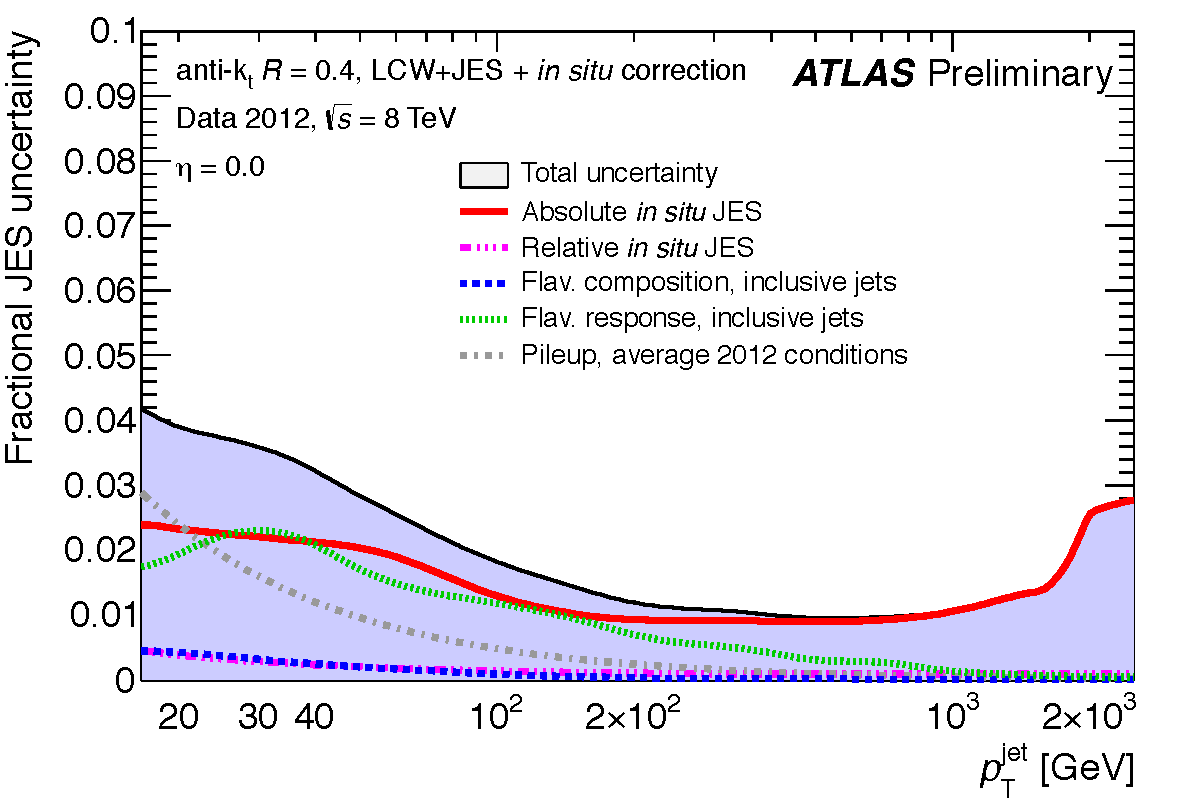
\includegraphics[width=0.6\textwidth]{fig/obj/smalljesunc.pdf}
\caption{The relative Jet Energy Scale (JES) uncertainty for jets in the region~\cite{JES}.}
\label{fig:jesex}
\end{figure}

\section{$b$-tagged Jets}
At the LHC, jets that contain $b$-quarks (called $b$-jets or $b$-tagged jets) can be distinguished from jets which only contain light quarks\cite{btagcom,btagptrel}. The long lifetime of $B$-hadrons is exploited to make this distinction. Because a $B$-hadron will travel a relatively long path through the detector before decaying, a \emph{secondary} vertex for this decay can be reconstructed and used to identify jets which contain a $b$-quark. The production of a top quark pair produces at least two $b$-jets (which are otherwise rare), so identifying $b$-jets leads to significant background reduction. 

At the ATLAS detector, several algorithms are used in conjunction to identify $b$-jets:
\begin{description}
\item[IP3D] is an impact parameter based algorithm that uses the tracks associated with the jet. First, tracks must pass quality cuts on the number of hits in the ID. Then, tracks are required to have $|d_0|< 1$ mm and $z_0<$ 1.5 mm in order to reject tracks from the decays of long-lived mesons, such as kaons, and photon conversion. These tracks are then associated to the jet with a jet \pt\ dependent \dR. Then, the algorithm uses the impact parameters' significance, $d_0/\sigma(d_0)$ and $z_0/\sigma(z_0)$, to produce the likelihood for tracks to originate from a $b$-jet. The likelihood distribution is produced from simulation.
\item[SV1] is an algorithm based on the secondary vertex. The tracks associated with the jet are required to pass quality cuts similar to IP3D. Next, all possible two-track vertices are considered. Vertices with masses compatible with long-lived particles like kaons or $\Lambda$ have both tracks removed from the list of associated tracks. Then, all remaining two-track vertices are combined into a single vertex and the track with the worst fit is removed. This procedure is repeated until the overall \chisq\ of the track errors to the vertex passes a quality threshold. Finally, a likelihood ratio technique is used to assign a $b$-tagging weight, using variables such as the secondary vertex mass, the number of two-track vertices, and the angle between the vertices and jet axis.

\item[JetFitterCombNN] uses the same tracks as IP3D. The algorithm attempts to find an axis and decay position of the $B$-hadron, including the possibility of an extra vertex due to a $D$-decay. A Kalman filter is used to start with the axis from the PV to the jet axis and update with addition of each track in the decay chain. The best combination of two vertices that fits the tracks is found. Then the decay length significance ($d_0/\sigma(d_0)$), the invariant mass of the tracks and the energy fraction of the tracks are combined into a neural network. The output of the neural network gives the likelihood that the jet is a light-, $c$-, or $b$-jet.
\end{description}




The results from these three algorithms, IP3D, SV1 and JetFitterCombNN, are combined into a single discriminant using a neural network with the MV1 $b$-tagger. The efficiency of these algorithms in rejecting light-jets and $c$-jets is shown in Figure~\ref{fig:btagEff}.

\begin{figure}[h]
\centering
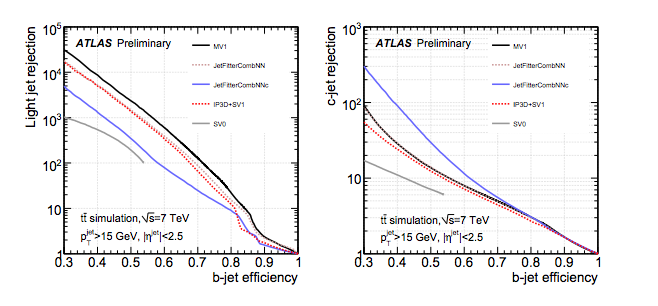
\includegraphics[width=0.9\textwidth]{fig/obj/btageff.png}
\caption{Light-jet rejection (left) and $c$-jet rejection (right) as a function of the $b$-tag efficiency for the
$b$-tagging algorithms discussed based on simulated \ttbar\ events.~\cite{btagptrel}.}
\label{fig:btagEff}
\end{figure}


